\documentclass[notheorems]{beamer}
% \documentclass{beamer}

\mode<presentation>
{
  % \usetheme{default}
  \usetheme{Antibes}
  \setbeamertemplate{footline}[frame number]{}
  \setbeamertemplate{navigation symbols}{}
}

\usepackage{amsmath}
\usepackage{amssymb}
\usepackage{ragged2e}
\usepackage{yhmath}
\usepackage{tikz}
\usepackage{centernot}
\usepackage{mleftright}
\let\left\mleft
\let\right\mright


% % \usepackage[utf8]{inputenc}
% \usepackage{pgfplots}
% % \DeclareUnicodeCharacter{2212}{−}
% % \usepgfplotslibrary{groupplots,dateplot}
% \usetikzlibrary{patterns,shapes.arrows}
% \pgfplotsset{compat=newest}

\justifying\let\raggedright\justifying

\makeatletter
\newenvironment<>{proofs}[1][\proofname]{
    \par
    \def\insertproofname{#1\@addpunct{.}}
    \usebeamertemplate{proof begin}#2}
  {\usebeamertemplate{proof end}}

  \newenvironment<>{solution}[1][Solution.]{
    \par
    \def\insertproofname{#1\@addpunct{.}}
    \usebeamertemplate{proof begin}#2}
  {\usebeamertemplate{proof end}}

  \newtheorem*{definition}{Definition}
  \newtheorem{example}{Example}[section]
  \newtheorem{theorem}{Theorem}[section]
  \newtheorem{property}{Property}[section]
\makeatother

\setbeamertemplate{theorems}[numbered]
% \setbeamertemplate{definition}[nonumbered]

\setbeamertemplate{section in toc}[sections numbered]
\setbeamertemplate{subsection in toc}[subsections numbered]
% \setbeamertemplate{subsubsection in toc}[subsubsections numbered]

\numberwithin{equation}{section}
\numberwithin{equation}{subsection}

\usefonttheme[onlymath]{serif}
\providecommand{\Arg}{\operatorname{Arg}}
\providecommand{\Ln}{\operatorname{Ln}}
\providecommand{\Arcsin}{\operatorname{Arcsin}}
\providecommand{\Arccos}{\operatorname{Arccos}}
\providecommand{\Arctan}{\operatorname{Arctan}}
\providecommand{\Arcsinh}{\operatorname{Arcsinh}}
\providecommand{\Arccosh}{\operatorname{Arccosh}}
\providecommand{\Arctanh}{\operatorname{Arctanh}}
\DeclareMathOperator{\dif}{d \!}

% \providecommand{\abs}[1]{\lvert#1\rvert}
% \providecommand{\abs}[1]{\left\lvert#1\right\rvert}
% \providecommand{\norm}[1]{\lVert#1\rVert}

\title{Chapter 4: Series}
\author{Taotao Wang, Associate Professor}
\institute{College of Electronics and Information Engineering, Shenzhen University}
\date{\today}

\begin{document}

\everymath{\displaystyle}

\begin{frame}
  \titlepage
\end{frame}

\begin{frame}{Outline}
  \tableofcontents
\end{frame}


\begin{frame}
	\textbf{Focus and Difficulty}
	\begin{itemize}
		\item Learning Focus: How to expand a function into Taylor series or Laurent series;
		\item Learning Difficulty: How to expand a function into Laurent series.
	\end{itemize}
\end{frame}


\section{Series}

\begin{frame}
  \frametitle{Outline}
  \tableofcontents[currentsection]
\end{frame}


%\begin{frame}
%  \begin{figure}
%    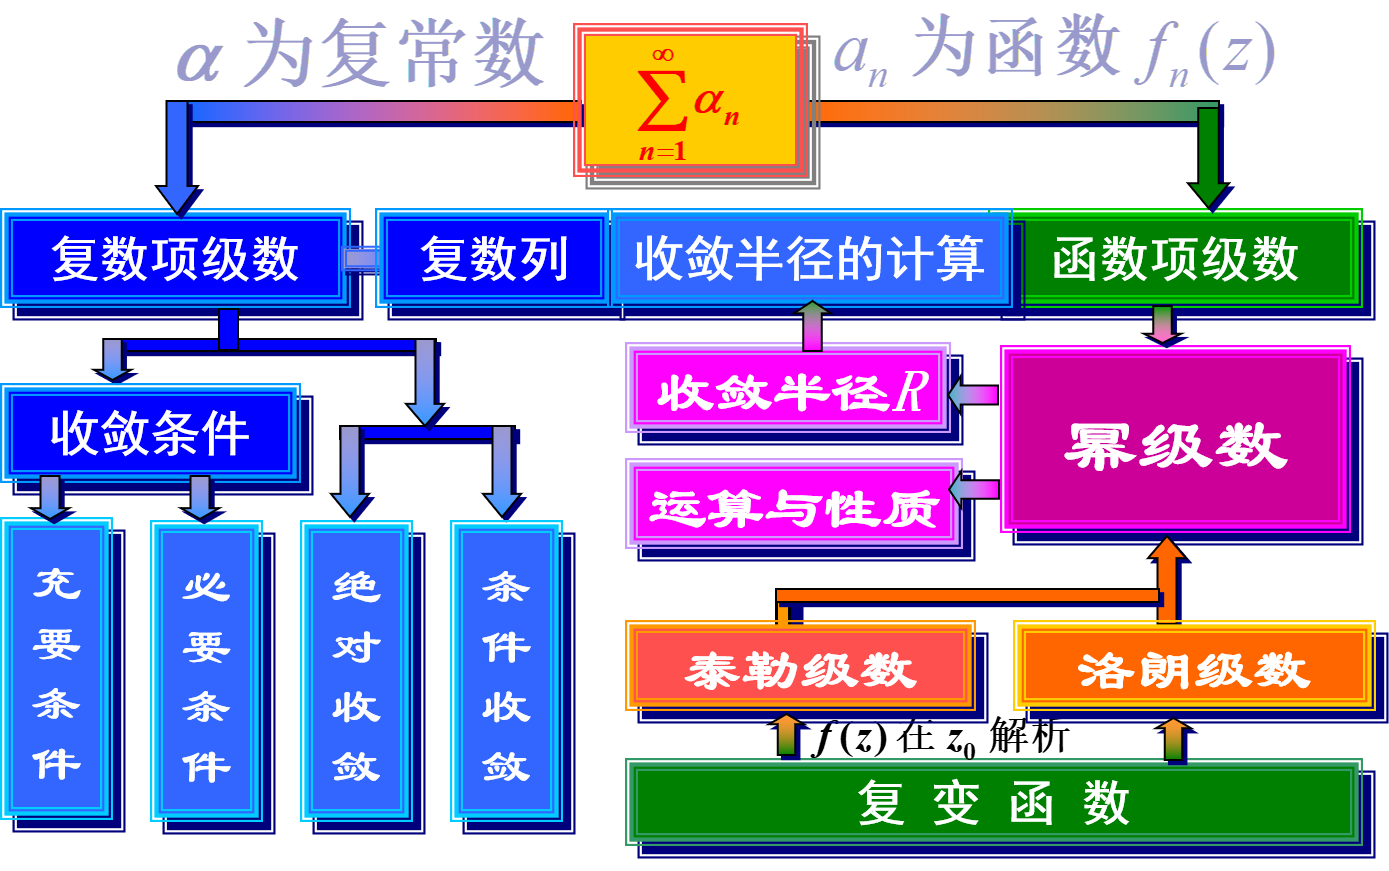
\includegraphics[width=\linewidth]{Figure_4_1_1.png}
%  \end{figure}
%\end{frame}



\begin{frame}
  \begin{enumerate}
    \item \textbf{Sequence of Complex Numbers}\\
          Let $\{\alpha_n\}(n=1,2,\cdots)$ be a sequence of complex numbers, where $\alpha_n=a_n+ib_n$ and $\alpha=a+ib$ be a certain complex number. If for any given $\varepsilon>0$, there exists a positive number $N(\varepsilon)$ related to $\varepsilon$ such that $|\alpha_n-\alpha|<\varepsilon$ is true when $n>N$, then $\alpha$ is said to be the limit of sequence $\{\alpha_n\}$ when $N \to \infty $ and we write
          \[\lim_{n\to\infty}\alpha_n=\alpha.\]
          We also say that sequence $\{\alpha_n\}$ converge to $\alpha$, if $\alpha$ is the limit of $\{\alpha_n\}$.
  \end{enumerate}
\end{frame}

\begin{frame}
  \begin{enumerate}
    \setcounter{enumi}{1}
    \item \textbf{Series of Complex Numbers}
          \begin{enumerate}[1)]
            \item Definition\\
                  Let $\{\alpha_n\}=\{a_n+ib_n\}$ be a sequence  of complex numbers. The summation expression
                  \[\sum_{n=1}^{\infty}\alpha_n=\alpha_1+\alpha_2+\cdots+\alpha_n+\cdots\]
                  denotes the infinite series of the complex numbers; and 
                  \[s_n=\alpha_1+\alpha_2+\cdots+\alpha_n\]
                  denotes the partial sum of the series. The partial sums itself is a sequence. 
          \end{enumerate}
  \end{enumerate}
\end{frame}

\begin{frame}
  \begin{enumerate}
    \item []
          \begin{enumerate}[1)]
            \setcounter{enumii}{1}
            \item Convergence and Divergence of Series of Complex Numbers\\
                  \begin{itemize}
                  	\item    If the partial sums of a series $s_n$ converges, the series $\sum_{n=1}^{\infty}\alpha_n$ converges, and the limit of the partial sums, $\lim_{n\to\infty}s_n=s$, is called the sum of the series; otherwise the series $\sum_{n=1}^{\infty}\alpha_n$ diverges.
                  	
                   \item  {\bf Necessary and sufficient condition}:\\
                  		Complex series $\sum_{n=1}^{\infty}\alpha_n$ converges $\Longleftrightarrow$ both real series $\sum_{n=1}^{\infty}a_n$ and $\sum_{n=1}^{\infty}b_n$ converge.
                  		
                  	\item {\bf Necessary condition}: $\sum_{n=1}^{\infty}\alpha_n$ converges $\Longrightarrow$ $\lim_{n\to\infty}\alpha_n=0$.
                  \end{itemize}



          \end{enumerate}
  \end{enumerate}
\end{frame}

\begin{frame}

  \begin{enumerate}
    \item []
          \begin{enumerate}[1)]
            \setcounter{enumii}{2}
            \item Absolute and Conditional Convergence of Series of Complex Numbers
            
            \begin{itemize}
            	\item  If a series $\sum_{n=1}^{\infty}|\alpha_n|$ converges, the series $\sum_{n=1}^{\infty}\alpha_n$ converges absolutely.
            	\item A convergent series, which is not absolutely convergent, is said to be conditionally convergent.
                \item $\sum_{n=1}^{\infty}\alpha_n$ is absolutely convergent $\Longleftrightarrow$ both $\sum_{n=1}^{\infty}a_n$ and $\sum_{n=1}^{\infty}b_n$ are absolutely convergent.
                \item  Absolute convergence of series $\begin{aligned}
                	\Longrightarrow \\
                	\centernot\Longleftarrow
                \end{aligned}$  Convergence of series.
            \end{itemize}



          \end{enumerate}
  \end{enumerate}
\end{frame}

\begin{frame}
  \begin{example}
    Does the following sequences converge? If it converges, find the limit.\\
    \begin{minipage}{0.5\linewidth}
      \begin{enumerate}
        \item $\alpha_n=\left(1+\frac{1}{n}\right)e^{i\frac{\pi}{n}}$;
      \end{enumerate}
    \end{minipage}\begin{minipage}{0.5\linewidth}
      \begin{enumerate}
        \setcounter{enumi}{1}
        \item $\alpha_n=n\cos in$.
      \end{enumerate}
    \end{minipage}
  \end{example}
  \begin{solution}<2->
    \begin{enumerate}
      \item $\alpha_n=\left(1+\frac{1}{n}\right)e^{i\frac{\pi}{n}}=\left(1+\frac{1}{n}\right)\left(\cos\frac{\pi}{n}+i\sin\frac{\pi}{n}\right)$,\\
            $a_n=\left(1+\frac{1}{n}\right)\cos\frac{\pi}{n}$, $b_n=\left(1+\frac{1}{n}\right)\sin\frac{\pi}{n}$.\\
            $\lim_{n\to\infty}a_n=1$, $\lim_{n\to\infty}b_n=0$.\\
            $\alpha_n$ is convergent, and $\lim_{n\to\infty}\alpha_n=1$.
      \item $\alpha_n=n\cos in=n\cosh n = {1 \over 2}n\left( {{e^n} + {e^{ - n}}} \right) $.\\
            When $n\to\infty$, $\alpha_n\to\infty$, $\alpha_n$ is not convergent.
    \end{enumerate}
  \end{solution}
\end{frame}

\begin{frame}
  \begin{example}
    Does the following series converge? Is it absolutely convergent?
    \begin{minipage}{0.33\linewidth}
      \begin{enumerate}
        \item $\sum_{n=1}^{\infty}\frac{1}{n}\left(1+\frac{i}{n}\right)$;
      \end{enumerate}
    \end{minipage}\begin{minipage}{0.3\linewidth}
      \begin{enumerate}
        \setcounter{enumi}{1}
        \item $\sum_{n=0}^{\infty}\frac{(8i)^n}{n!}$;
      \end{enumerate}
    \end{minipage}\begin{minipage}{0.37\linewidth}
      \begin{enumerate}
        \setcounter{enumi}{2}
        \item $\sum_{n=1}^{\infty}\left[\frac{(-1)^n}{n}+\frac{1}{2^n}i\right]$.
      \end{enumerate}
    \end{minipage}
  \end{example}
  \begin{solution}<2->
    \begin{enumerate}
      \item Because $\sum_{n=1}^{\infty}a_n=\sum_{n=1}^{\infty}\frac{1}{n}$ diverges and $\sum_{n=1}^{\infty}b_n=\sum_{n=1}^{\infty}\frac{1}{n^2}$ converges, the original series diverges.
    \end{enumerate}
  \end{solution}
\end{frame}

\begin{frame}
  \begin{solution}[Solution\ (Cont.)]
    \begin{enumerate}
      \setcounter{enumi}{1}
      \item Because $\left|\frac{(8i)^n}{n!}\right|=\frac{8^n}{n!}$ and the ratio test tells us that $\sum_{n=1}^{\infty}x_n=\frac{8^n}{n!}$ converges, the original series is convergent and absolutely convergent.
      \item Because both $\sum_{n=1}^{\infty}\frac{(-1)^n}{n}$ and $\sum_{n=1}^{\infty}\frac{1}{2^n}$ converge, the original series converges. Because $\sum_{n=1}^{\infty}\frac{(-1)^n}{n}$ is conditionally convergent, the original series is not absolutely convergent.
    \end{enumerate}
  \end{solution}
\end{frame}

\begin{frame}
  \begin{enumerate}
    \setcounter{enumi}{2}
    \item \textbf{Series of Complex Functions}\\
          Let $\{f_n(z)\}(n=1,2,\cdots)$ be a sequence of complex functions, each of which is defined in the domain $D$. Then, the summation expression 
          \[\sum_{n=1}^{\infty}f_n(z)=f_1(z)+f_2(z)+\cdots+f_n(z)+\cdots\]
          denotes the series of complex functions; and 
          \[s_n(z)=f_1(z)+f_2(z)+\cdots+f_n(z)\]
          denotes the partial sum of the series. The limit of the partial sums $s_n(z)$ (if it exists) is called the sum of the series or sum function. 
  \end{enumerate}
\end{frame}

\begin{frame}
  \begin{enumerate}
    \setcounter{enumi}{3}
    \item \textbf{Power Series}
          \begin{enumerate}[1)]
            \item Definition\\
                  A series of functions having the form
                  \[\sum_{n=0}^{\infty}c_n(z-a)^n=c_0+c_1(z-a)+c_2(z-a)^2+\cdots+c_n(z-a)^n+\cdots\]
                  is called a power series.\\
                  When $a=0$, we have  $\sum_{n=0}^{\infty}c_nz^n=c_0+c_1z+c_2z^2+\cdots+c_nz^n+\cdots$.
          \end{enumerate}
  \end{enumerate}
\end{frame}

\begin{frame}
  \begin{enumerate}
    \item []
          \begin{enumerate}[1)]
            \setcounter{enumii}{1}
            \item Convergence Theorem
          \end{enumerate}
  \end{enumerate}
  \begin{theorem}[Abel's Theorem]
    If a power series $\sum_{n=0}^{\infty}c_nz^n$ is convergent at the point $z_1$, then it is absolutely convergent in any open disk $|z|<|z_1|$.\\
    If the series $\sum_{n=0}^{\infty}c_nz^n$ is divergent at a point $z_2$, then it is divergent in the domain $|z|>|z_2|$.
  \end{theorem}
\end{frame}

\begin{frame}
  \begin{enumerate}
    \item []
          \begin{enumerate}[1)]
            \setcounter{enumii}{2}
            \item Convergence Circle and Convergence Radius\\
                  For any power series, its convergence radius must be one of following three cases:\\
                  \begin{enumerate}[i]
                    \item It converges only at $z=0$, and it convergence radius is $0$;
                    \item It converges in the entire $z$-plane, and it convergence radius is $\infty $;
                    \item There exists a convergence radius $R>0$, when $|z|<R$ it converges, when $|z|>R$ it diverges.
                  \end{enumerate}
          \end{enumerate}
  \end{enumerate}
\end{frame}

\begin{frame}
  \begin{center}
    \begin{tikzpicture}[scale=2]
      \fill [cyan] (-1,-1) rectangle (1,1);
      \node [circle,draw=red,fill=green,minimum size=80] (C) at (0,0){};
      \draw [->] (-1.2,0) -- (1.2,0) node [right] {$x$};
      \draw [->] (0,-1.2) -- (0,1.2) node [right] {$y$};
      \node [below left] at (0,0) {$O$};
      \draw [->] (0,0) -- node [below right] (R) {$R$} (C.north east);
      \draw node (a) at (2,0.5) {radius of convergence};
      \draw [-] (a) -- (R);
      \draw node (b) at (2,-0.5) {circle of convergence};
      \draw [-] (b) -- (C.south east);
    \end{tikzpicture}
  \end{center}
  Note: The convergence and divergence of a power series on convergent circle is uncertain, which requires specific analysis of the power series.
\end{frame}

\begin{frame}
  \begin{example}
    Find the radius of convergence and the sum of the series $\sum_{n=0}^{\infty}z^n=1+z+z^2+\cdots+z^n+\cdots$.
  \end{example}
  \begin{solution}<2->
    $s_n=1+z+z^2+\cdots+z^n=\frac{1-z^n}{1-z}\quad(z\neq 1)$.\\
    When $|z|<1$, because $\lim_{n\to\infty}z^n=0$, that is $\lim_{n\to\infty}s_n=\frac{1}{1-z}$, the series converges, the sum of the series is $\frac{1}{1-z}$. When $|z|\geq 1$, because $z^n$ does not approach zero when $n\to\infty$, the series diverges.\\
    The region of convergence is $|z|<1$, within this region the series is absolutely convergent, and $\frac{1}{1-z}=1+z+z^2+\cdots+z^n+\cdots$.
  \end{solution}
\end{frame}

\begin{frame}
  \begin{enumerate}
    \item []
          \begin{enumerate}[1)]
            \setcounter{enumii}{3}
            \item Methods of Finding the Radius of Convergence\\
                  \begin{enumerate}[i]
                    \item By using ratio test:\\
                          If $\lim_{n\to\infty}\left|\frac{c_{n+1}}{c_n}\right|=\lambda\neq 0$, the radius of convergence is $R=\frac{1}{\lambda}$.
                    \item By using root test:\\
                          If $\lim_{n\to\infty}\sqrt[n]{|c_n|}=\lambda\neq 0$, the radius of convergence is $R=\frac{1}{\lambda}$.\\
                          That is $R=\begin{cases}
                              \frac{1}{\lambda}, & 0<\lambda<+\infty; \\
                              +\infty,           & \lambda=0;         \\
                              0,                 & \lambda=+\infty.
                            \end{cases}$
                  \end{enumerate}
          \end{enumerate}
  \end{enumerate}
\end{frame}

\begin{frame}
  \begin{example}
    Find the radius of convergence of the following power series:
    \begin{enumerate}
      \item $\sum_{n=1}^{\infty}\frac{z^n}{n^3}$ (Determine the convergence on the convergence circle);
      \item $\sum_{n=1}^{\infty}\frac{(z-1)^n}{n}$ (Determine the convergence at point $z=0,2$);
      \item $\sum_{n=0}^{\infty}(\cos in)z^n$.
    \end{enumerate}
  \end{example}
\end{frame}

\begin{frame}
  \begin{solution}
    \begin{enumerate}
      \item Because $\lim_{n\to\infty}\left|\frac{c_{n+1}}{c_n}\right|=\lim_{n\to\infty}\left(\frac{n}{n+1}\right)^3=1$\\
            (or $\lim_{n\to\infty}\sqrt[n]{|c_n|}=\lim_{n\to\infty}\sqrt[n]{\frac{1}{n^3}}=\lim_{n\to\infty}\frac{1}{\sqrt[n]{n^3}}=1$),\\
            the radius of convergence is $R=1$.\\
            That means that the  power series converges inside the circle $|z|=1$ and diverges outside the circle. Because when $|z|=1$, $\sum_{n=1}^{\infty}\left|\frac{z^n}{n^3}\right|=\sum_{n=1}^{\infty}\frac{1}{n^3}$ is a $p$-series and $p=3>1$, the series is convergent everywhere on the convergence circle.
    \end{enumerate}
  \end{solution}
\end{frame}

\begin{frame}
  \begin{solution}[Solution\ (Cont.)]
    \begin{enumerate}
      \setcounter{enumi}{1}
      \item Because $\lim_{n\to\infty}\left|\frac{c_{n+1}}{c_n}\right|=\lim_{n\to\infty}\frac{n}{n+1}=1$, that is $R=1$.\\
            On the convergence circle  $|z-1|=1$, when $z=0$, the series becomes $\sum_{n=1}^{\infty}(-1)^n\frac{1}{n}$ and it converges; when $z=2$, the series becomes $\sum_{n=1}^{\infty}\frac{1}{n}$ and it diverges. This example shows that there are convergence points and divergence points on the convergence circle.
      \item Because $c_n=\cos in=\cosh n=\frac{1}{2}\left(e^n+e^{-n}\right)$, $\lim_{n\to\infty}\left|\frac{c_{n+1}}{c_n}\right|=\lim_{n\to\infty}\frac{e^{n+1}+e^{-n-1}}{e^n+e^{-n}}=e$, the convergence radius is $R=\frac{1}{e}$.
    \end{enumerate}
  \end{solution}
\end{frame}

\begin{frame}
  \begin{enumerate}
    \item []
          \begin{enumerate}[1)]
            \setcounter{enumii}{4}
            \item Operation and properties of power series\\
                  Let $f(z)=\sum_{n=0}^{\infty}a_nz^n,R=r_1,\quad g(z)=\sum_{n=0}^{\infty}b_nz^n,R=r_2$.\\
                  \begin{itemize}
                    \item $\begin{aligned}[t]
                              f(z)\pm g(z) & =\sum_{n=0}^{\infty}a_nz^n\pm\sum_{n=0}^{\infty}b_nz^n \\
                                           & =\sum_{n=0}^{\infty}(a_n\pm b_n)z^n,\ R=\min(r_1,r_2).
                            \end{aligned}$\\
                      \item  $\begin{aligned}[t]
                              f(z)\cdot g(z) & =\left(\sum_{n=0}^{\infty}a_nz^n\right)\cdot\left(\sum_{n=0}^{\infty}b_nz^n\right) \\
                                             & =\sum_{n=0}^{\infty}(a_nb_0+a_{n-1}b_1+\cdots+a_0b_n)z^n, R=\min(r_1,r_2)
                            \end{aligned}$
                  \end{itemize}
          \end{enumerate}
  \end{enumerate}
\end{frame}

\begin{frame}
  \begin{enumerate}
    \item []
          \begin{enumerate}[1)]
           \setcounter{enumii}{5}
             \item Compound operation of power series\\
 
             When $|z|<r$, we have $f(z)=\sum_{n=0}^{\infty}a_nz^n$. And $g(z)$ is analytic in $|z|<R$ and $|g(z)|<r$. Then  $f\big[g(z)\big]=\sum_{n=0}^{\infty}a_n\big[g(z)\big]^n$, when $|z|<R$.
              
                
          \end{enumerate}
  \end{enumerate}
\end{frame}

\begin{frame}
  \begin{enumerate}
    \item []
          \begin{enumerate}[1)]
          	\setcounter{enumii}{6}
          	\item The integral and derivative of complex power series inside the convergence circle. \\ 
            Let $f(z)=\sum_{n=0}^{\infty}c_n(z-a)^n$ be analytic inside the convergence circle of  $|z-a|=R$.     
             \begin{itemize}
                    \item The derivative of $f(z)$ in the convergence circle can be obtained by taking the derivative of its power series term by term.
                          \[f'(z)=\sum_{n=1}^{\infty}nc_n(z-a)^{n-1},|z-a|<R\]
                    \item $f(z)$ can be integrated term by term in the convergence circle.
                          \[\int_C f(z)\dif z=\sum_{n=0}^{\infty}c_n\int_C (z-a)^n\dif z,\ C:|z-a|=r<R\]
                          \[\text{or}\ \int_a^z f(\xi)\dif\xi=\sum_{n=0}^{\infty}\frac{c_n}{n+1}(z-a)^{n+1}\]
                          where $C$ is any curve connecting points $a$ and $z$ in the convergence circle.
                  \end{itemize}
          \end{enumerate}
  \end{enumerate}
\end{frame}

\section{Taylor Series}

\begin{frame}
  \frametitle{Outline}
  \tableofcontents[currentsection]
\end{frame}

%\begin{frame}
%  \begin{figure}
%    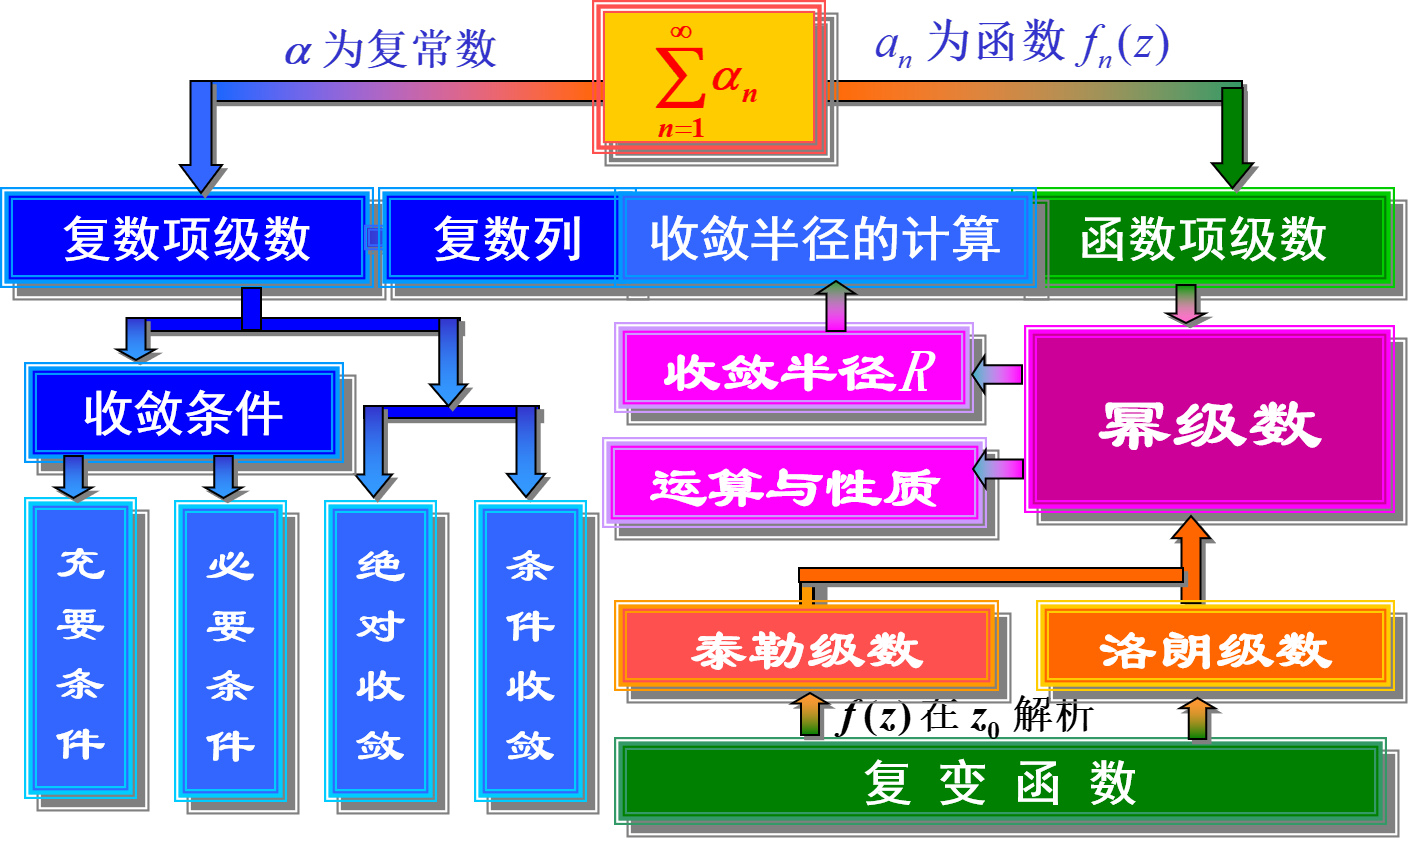
\includegraphics[width=\linewidth]{Figure_4_2_1.png}
%  \end{figure}
%\end{frame}

\begin{frame}
  \begin{block}{Review 1}
    \begin{itemize}
      \item Power series\\
            $\sum_{n=0}^{\infty}c_n(z-z_0)^n=c_0+c_1(z-z_0)+\cdots+c_n(z-z_0)^n+\cdots$
      \item Abel's theorem
            \begin{enumerate}
              \item \resizebox*{\linewidth}{!}{$\sum_{n=0}^{\infty}c_nz_0^n\ (z_0\neq 0)$ converges $\Longrightarrow$ $\sum_{n=0}^{\infty}c_nz^n\ (|z|<|z_0|)$ absolutely converges}
              \item $\sum_{n=0}^{\infty}c_nz_0^n$ diverges $\Longrightarrow$ $\sum_{n=0}^{\infty}c_nz^n\ (|z|>|z_0|)$ diverges
            \end{enumerate}
      \item Convergence region is determined by a circle $C_R:|z|=R$, where $R$ is called the convergence radius.
      \item It converges inside $C_R$, diverges outside $C_R$, and its convergence is uncertain on $C_R$.
    \end{itemize}
  \end{block}
\end{frame}

\begin{frame}
  \begin{block}{Review 2}
    Methods of Finding Convergence Radius
    \begin{enumerate}
      \item By using ratio test:\\
            If $\lim_{n\to\infty}\left|\frac{c_{n+1}}{c_n}\right|=l$, the radius of convergence is $R=\frac{1}{l}$.
      \item By using root test:\\
            If $\lim_{n\to\infty}\sqrt[n]{|c_n|}=l$, the radius of convergence is $R=\frac{1}{l}$.
    \end{enumerate}
    \ \\
    $l=0\Longrightarrow R=\infty$, the power series is convergent everywhere.\\
    \resizebox*{\linewidth}{!}{$l=\infty\Longrightarrow R=0$, the power series is divergent everywhere except 0.}
  \end{block}
\end{frame}

\begin{frame}
  \begin{block}{Review 3}
    The convergence radius of power series $\sum_{n=0}^{\infty}c_n(z-z_0)^n$ is $R$, its sum function is $f(z)=\sum_{n=0}^{\infty}c_n(z-z_0)^n$.
    \begin{enumerate}
      \item The sum function is analytic inside the convergence circle.
      \item The derivative of $f(z)$ in the convergence circle can be obtained by taking the derivative of its power series term by term.
            \begin{center}
              $f'(z)=\sum_{n=1}^{\infty}nc_n(z-a)^{n-1},|z-a|<R$
            \end{center}
      \item $f(z)$ can be integrated term by term in the convergence circle: $\int_C f(z)\dif z=\sum_{n=0}^{\infty}c_n\int_C (z-a)^n\dif z,\ C:|z-a|<R$
    \end{enumerate}
  \end{block}
\end{frame}

\begin{frame}
  \begin{block}{Review 4}
    \begin{itemize}
      \item Taylor series: If the function $f(x)$ has derivatives of order up to $(n+1)$ in a neighborhood of a point $x_0$, then the Taylor series of order $n$ of $f(x)$ in that neighborhood is:\\
            \resizebox*{\linewidth}{!}{$f(x)=f(x_0)+f'(x_0)(x-x_0)+\frac{f''(x_0)}{2!}(x-x_0)^2+\cdots+\frac{f^{(n)}(x_0)}{n!}(x-x_0)^n+R_n(x)$}
      \item $R_n(x)=\frac{f^{(n+1)}(\epsilon)}{(n+1)!}(x-x_0)^{n+1}$ is called Lagrange remainder, where $\epsilon \in (x,x_0)$
      \item When $x_0=0$, the power series is called Maclaurin series.
      \item Review Cauchy's integral formula for derivatives.
    \end{itemize}
  \end{block}
\end{frame}

\begin{frame}
  \begin{block}{Question}
    \begin{enumerate}
      \item Why do we study power series?
      \item Can any analytic function be expressed in power series?
    \end{enumerate}
  \end{block}
\end{frame}

\begin{frame}
  \begin{enumerate}
    \item \textbf{Motivation}\\
          Let $f(z)$ be an analytic function in domain $D$ and $r=|\zeta-z_0|$ be any circle centered on $z_0$ in $D$, called $K$. We take an any point $z$ inside $K$. 
          \begin{center}
            \begin{tikzpicture}
              \draw plot[smooth cycle] coordinates{(-0.5,1.2) (1.5,0.7) (1.8,-0.7) (-0.6,-1.5) (-2,-1)};
              \draw (0,0) circle[radius=1];
              \node [circle,fill=red,scale=0.2] (z_0) at (0,0) {};
              \node [below left] at (z_0) {$z_0$};
              \node [circle,fill=red,scale=0.2] (z) at (0.2,0.6) {};
              \node (z_name) [right] at (z) {$z$};
              \node [circle,fill=red,scale=0.2] (zeta) at (0.707,-0.707) {};
              \node [below left] at (-0.707,-0.707) {$D$};
              \node [right] at (zeta) {$\zeta$};
              \node (K_name) [below right] at (1,0) {$K$};
              \draw [->] (z_0) -- node [above] {$r$} (1,0);
              \draw [-] (z_name) -- (2,0.6) node [right] {any point in $K$};
              \draw [-] (K_name) -- (2,-0.7) node [right] {circle $|\zeta-z_0|=r$};
            \end{tikzpicture}
          \end{center}
  \end{enumerate}
\end{frame}

\begin{frame}
  \begin{enumerate}
    \item []
          According to Cauchy's integral formula,\\
          $f(z)=\frac{1}{2\pi i}\oint_K \frac{f(\zeta)}{\zeta-z}\dif\zeta$, where $K$ is taken counterclockwise.\\
          $\vdots$\\
          So $\left|\frac{z-z_0}{\zeta-z_0}\right|<1$ and $\frac{1}{\zeta-z}=\frac{1}{\zeta-z_0}\frac{1}{1-\frac{z-z_0}{\zeta-z_0}}$.
  \end{enumerate}
\end{frame}

\begin{frame}
  \begin{enumerate}
    \item []
          \resizebox*{\linewidth}{!}{
            $\begin{aligned}
                \frac{1}{\zeta-z} & =\frac{1}{\zeta-z_0}\frac{1}{1-\frac{z-z_0}{\zeta-z_0}}                                                                                                             \\
                                  & =\frac{1}{\zeta-z_0}\left[1+\left(\frac{z-z_0}{\zeta-z_0}\right)+\left(\frac{z-z_0}{\zeta-z_0}\right)^2+\cdots+\left(\frac{z-z_0}{\zeta-z_0}\right)^n+\cdots\right] \\
                                  & =\sum_{n=0}^{\infty}\frac{1}{(\zeta-z_0)^{n+1}}(z-z_0)^n.
              \end{aligned}$
          }\\
          So $\begin{aligned}[t]
              f(z)= & \sum_{n=0}^{N-1}\left[\frac{1}{2\pi i}\oint_K \frac{f(\zeta)}{(\zeta-z_0)^{n+1}}\dif\zeta\right](z-z_0)^n     \\
                    & +\frac{1}{2\pi i}\oint_K\left[\sum_{n=N}^{\infty}\frac{f(\zeta)}{(\zeta-z_0)^{n+1}}(z-z_0)^n\right]\dif\zeta.
            \end{aligned}$
  \end{enumerate}
\end{frame}

\begin{frame}
  \begin{enumerate}
    \item []
          According to Cauchy's integral formula for derivatives,\\
          the above equation can be written as\\
          $\sum_{n=0}^{N-1}\frac{f^{(n)}(z_0)}{n!}(z-z_0)^n+R_N(z)$,\\
          where $R_N(z)=\frac{1}{2\pi i}\oint_K\left[\sum_{n=N}^{\infty}\frac{f(\zeta)}{(\zeta-z_0)^{n+1}}(z-z_0)^n\right]\dif\zeta$.\\
          If $\lim_{N\to\infty}R_N(z)=0$,\\
          we have $f(z)=\sum_{n=0}^{\infty}\frac{f^{(n)}(z_0)}{n!}(z-z_0)^n$ inside $K$, which means that $f(z)$ in $K$ can be expressed as a power series.
         
  \end{enumerate}
\end{frame}

\begin{frame}
  \begin{enumerate}
    \item []
    We now prove that  $\lim_{N\to\infty}R_N(z)=0$, where \\$R_N(z)=\frac{1}{2\pi i}\oint_K\left[\sum_{n=N}^{\infty}\frac{f(\zeta)}{(\zeta-z_0)^{n+1}}(z-z_0)^n\right]\dif\zeta$.\\
          Let $\left|\frac{z-z_0}{\zeta-z_0}\right|=\frac{|z-z_0|}{r}=q$,\\
          where $q$ is independent of the integral variable and $0\leq q<1$.\\
          Since $f(z)$ is analytic in $D$ $(K\subset D)$,
          $f(\zeta)$ is continuous and bounded on $K$.
  \end{enumerate}
\end{frame}

\begin{frame}
  \begin{enumerate}
    \item []
          Thus, there exists a positive number $M$, such that $|f(\zeta)\leq M|$ on $K$.\\
          $\begin{aligned}
              |R_N(z)| & \leq\frac{1}{2\pi}\oint_K\left|\sum_{n=N}^{\infty}\frac{f(\zeta)}{(\zeta-z_0)^{n+1}}(z-z_0)^n\right|\dif\zeta                          \\
                       & \leq\frac{1}{2\pi}\oint_K\left[\sum_{n=N}^{\infty}\frac{|f(\zeta)|}{|\zeta-z_0|}\left|\frac{z-z_0}{\zeta-z_0}\right|^n\right]\dif\zeta \\
                       & \leq\frac{1}{2\pi}\cdot\sum_{n=N}^{\infty}\frac{M}{r}q^n\cdot2\pi r=\frac{Mq^N}{1-q}.
            \end{aligned}$
  \end{enumerate}
\end{frame}

\begin{frame}
  \begin{enumerate}
    \item []
          $\lim_{N\to\infty}q^N=0\Longrightarrow\lim_{N\to\infty}R_N(z)=0$ holds inside $K$.\\
          Therefore, we get $f(z)=\sum_{n=0}^{\infty}\frac{f^{(n)}(z_0)}{n!}(z-z_0)^n$ inside $K$,\\
          which is called the Taylor series of $f(z)$ with center at $z=z_0$.\\
          {\color{blue}The radius of the circle $K$ can increase arbitrarily, as long as $K$ is in $D$}.
  \end{enumerate}
\end{frame}

%\begin{frame}
%  \begin{example}
%    Let $f(z)$ be analytic in domain $0<|z-z_0|<R$, $f(z)=\sum_{n=-\infty}^{+\infty}c_n(z-z_0)^n$, where $c_n=\underline{\makebox[50pt]{}}$.
%    \begin{enumerate}[A]
%      \item $\frac{f^{(n)}(z_0)}{n!},\ n=0,1,2,\cdots;$
%      \item $\frac{f^{(n)}(z_0)}{n!},\ n=0,\pm 1,\pm 2,\cdots;$
%      \item $\frac{1}{2\pi i}\oint_C \frac{f(\zeta)}{(\zeta-z_0)^{n+1}}\dif\zeta,\ n=0,\pm 1,\pm 2,\cdots,$\\
%            where $C$ is any closed curve around $z_0$ in a ring domain $;$
%      \item $2\pi i\frac{f^{(n)}(z_0)}{n!},\ n=0,1,2,\cdots.$
%    \end{enumerate}
%  \end{example}
%\end{frame}

\begin{frame}
  \begin{enumerate}
    \item []
          \begin{center}
            \begin{tikzpicture}
              \draw plot[smooth cycle] coordinates{(-0.5,1.2) (1.5,0.7) (1.8,-0.7) (-0.6,-1.5) (-2,-1)};
              \draw (0,0) circle[radius=1];
              \node [circle,fill=red,scale=0.2] (z_0) at (0,0) {};
              \node [below left] at (z_0) {$z_0$};
              \node [circle,fill=red,scale=0.2] (z) at (0.2,0.6) {};
              \node (z_name) [right] at (z) {$z$};
              \node [circle,fill=red,scale=0.2] (zeta) at (0.707,-0.707) {};
              \node [below left] at (-0.707,-0.707) {$D$};
              \node [right] at (zeta) {$\zeta$};
              \node (K_name) [below right] at (1,0) {$K$};
              \draw [->] (z_0) -- node [above] {$r$} (1,0);
              \draw [-] (z_name) -- (2,0.6) node [right] {any point in $K$};
              \draw [-] (K_name) -- (2,-0.7) node [right] {circle $|\zeta-z_0|=r$};
              \draw [dashed,red] (0,0) -- (0,1.2);
              \node [left,red] at (0,0.5) {$d$};
            \end{tikzpicture}
          \end{center}
          Let $d$ be the shortest distance from $z_0$ to any point on the boundary of $D$, the Taylor series of $f(z)$ at $z=z_0$ holds in $|z-z_0|<d$. Because any $z$ satisfies $|z-z_0|<d$ can make $f(z)=\sum_{n=0}^{\infty}\frac{f^{(n)}(z_0)}{n!}(z-z_0)^n$ holds, that is $R\geq d$.\\
          Taylor's theorem is obtained from above.
  \end{enumerate}
\end{frame}

\begin{frame}
  \begin{enumerate}
    \setcounter{enumi}{1}
    \item \textbf{Taylor's Theorem}
  \end{enumerate}
  \begin{theorem}
    Let $f(z)$ be analytic in domain $D$, $z_0$ be a point in $D$ and $d$ be the shortest distance from $z_0$ to any point on the boundary of $D$.\\
    When $|z-z_0|<d$, there is
    \[f(z)=\sum_{n=0}^{\infty}c_n(z-z_0)^n,\]
    where $c_n=\frac{1}{n!}f^{(n)}(z_0),\ n=0,1,2,\cdots$.
  \end{theorem}
\end{frame}

\begin{frame}
  \begin{block}{Note}
    \begin{enumerate}
      \item The requirement of Taylor series of complex functions is much weaker than that of real functions. {\color{blue}(Why?)}
      \item If $f(z)$ has singularities in $D$, $d=|\alpha-z_0|$, where $\alpha$ is the closest singularity to $z_0$.
      \item When $z_0=0$, the series is also called a Maclaurin series.
      \item The Taylor series of any analytic function at one point is unique. {\color{blue}(Why?)}
    \end{enumerate}
  \end{block}
\end{frame}

\begin{frame}
  \begin{block}{Note}
    Because an analytic $f(z)$ can guarantee the existence of any order derivatives, the use of Taylor series of complex function is much wider than that of real function.
  \end{block}
\end{frame}

\begin{frame}
  \begin{block}{Question}
    Using Taylor series, the function can be expanded into power series. Is the expansion unique?
  \end{block}
  \begin{block}{Answer}
    Let $f(z)$ be expanded into a power series at $z_0$:\\
    $f(z)=a_0+a_1(z-z_0)+a_2(z-z_0)^2+\cdots+a_n(z-z_0)^n+\cdots$.\\
    Then $f(z_0)=a_0,f'(z_0)=a_1,\cdots$,\\
    that is $a_n=\frac{1}{n!}f^{(n)}(z_0)$.\\
    Therefore, the result of any analytic function expanded into power series is Taylor series. It is unique.
  \end{block}
\end{frame}

\begin{frame}
  \begin{enumerate}
    \setcounter{enumi}{2}
    \item \textbf{Expand Function as a Taylor Series}
          \begin{enumerate}[1)]
            \item Direct Method\\
                  Using Taylor's theorem, the coefficients can be calculated directly:
                  \[c_n=\frac{1}{n!}f^{(n)}(z_0),\ n=0,1,2,\cdots\]
          \end{enumerate}
  \end{enumerate}
\end{frame}

\begin{frame}
  \begin{example}
    Find the Taylor series for $e^z$ at the point $z=0$.
  \end{example}
  \begin{solution}<2->
    Because $\left(e^z\right)^{(n)}=e^z$, $\left.\left(e^z\right)^{(n)}\right|_{z=0}=1,\ (n=0,1,2,\cdots)$,\\
    $e^z=1+z+\frac{z^2}{2!}+\cdots+\frac{z^n}{n!}+\cdots=\sum_{n=0}^{\infty}\frac{z^n}{n!}$.\\
    Because $e^z$ is analytic everywhere in the complex plane,\\
    the radius of convergence of the series is $R=\infty$.
  \end{solution}
\end{frame}

\begin{frame}
  \begin{example}
    Find the Taylor series for $\sin z$ and $\cos z$ at the point $z=0$.
  \end{example}
  \begin{solution}<2->
    According to the example above and we have\\
    $\sin z=z-\frac{z^3}{3!}+\frac{z^5}{5!}-\cdots+(-1)^n\frac{z^{2n+1}}{(2n+1)!}+\cdots,\ (R=\infty)$\\
    $\cos z=1-\frac{z^2}{2!}+\frac{z^4}{4!}-\cdots+(-1)^n\frac{z^{2n}}{(2n)!}+\cdots,\ (R=\infty)$
  \end{solution}
\end{frame}

\begin{frame}
  \begin{enumerate}
    \item []
          \begin{enumerate}[1)]
            \setcounter{enumii}{1}
            \item Indirect Method\\
                  We can use the power series expansion of some known functions, and then use the operational and analytical properties of the power series to obtain the power series expansion of the given function.\\
                  Advantages: There is no need to find all derivatives and convergence radius. Thus, it is simpler and more widely used than the direct expansion.
          \end{enumerate}
  \end{enumerate}
\end{frame}

\begin{frame}
  \begin{example}
    Find the Taylor series for $\sin z$ at the point $z=0$ by using indirect method.
  \end{example}
  \begin{solution}<2->
    $\begin{aligned}
        \sin z & =\frac{1}{2i}\left(e^{iz}-e^{-iz}\right)                                                             \\
               & =\frac{1}{2i}\left[\sum_{n=0}^{\infty}\frac{(iz)^n}{n!}-\sum_{n=0}^{\infty}\frac{(-iz)^n}{n!}\right] \\
               & =\sum_{n=0}^{\infty}(-1)^n\frac{z^{2n+1}}{(2n+1)!}
      \end{aligned}$
  \end{solution}
\end{frame}

\begin{frame}
  \begin{block}{Taylor expansion of common functions}
    \begin{enumerate}
      \item $e^z=1+z+\frac{z^2}{2!}+\cdots+\frac{z^n}{n!}+\cdots=\sum_{n=0}^{\infty}\frac{z^n}{n!},\ (|z|<\infty)$
      \item $\frac{1}{1-z}=1+z+z^2+\cdots+z^n+\cdots=\sum_{n=0}^{\infty}z^n,\ (|z|<1)$
      \item \resizebox*{\linewidth}{!}{$\frac{1}{1+z}=1-z+z^2-\cdots+(-1)^nz^n+\cdots=\sum_{n=0}^{\infty}(-1)^nz^n,\ (|z|<1)$}
      \item $\sin z=z-\frac{z^3}{3!}+\frac{z^5}{5!}-\cdots+(-1)^n\frac{z^{2n+1}}{(2n+1)!}+\cdots,\ (|z|<\infty)$
    \end{enumerate}
  \end{block}
\end{frame}

\begin{frame}
  \begin{block}{Taylor expansion of common functions}
    \begin{enumerate}
      \setcounter{enumi}{4}
      \item $\cos z=1-\frac{z^2}{2!}+\frac{z^4}{4!}-\cdots+(-1)^n\frac{z^{2n}}{(2n)!}+\cdots,\ (|z|<\infty)$
      \item $\begin{aligned}[t]
                \ln(1+z) & =z-\frac{z^2}{2}+\frac{z^3}{3}-\cdots+(-1)^n\frac{z^{n+1}}{n+1}+\cdots \\
                         & =\sum_{n=0}^{\infty}(-1)^n\frac{z^{n+1}}{n+1},\ (|z|<1)
              \end{aligned}$
      \item $\begin{aligned}[t]
                (1+z)^\alpha= & 1+\alpha z+\frac{\alpha(\alpha-1)}{2!}z^2+\frac{\alpha(\alpha-1)(\alpha-2)}{3!}z^3+\cdots \\
                              & +\frac{\alpha(\alpha-1)\cdots(\alpha-n+1)}{n!}z^n+\cdots,\ (|z|<1)
              \end{aligned}$
    \end{enumerate}
  \end{block}
\end{frame}

\begin{frame}
  \begin{enumerate}
    \setcounter{enumi}{3}
    \item \textbf{Example}
  \end{enumerate}
  \begin{example}
    Represent $\frac{1}{(1+z)^2}$ as a power series of $z$.
  \end{example}
  \begin{solution}<2->
    Because $\frac{1}{(1+z)^2}$ has a singularity $z=-1$ on $|z|=1$ and it is analytic inside the circle $|z|<1$, it can be expanded into a power series.\\
    $\frac{1}{1+z}=1-z+z^2-\cdots+(-1)^nz^n+\cdots,\ (|z|<1)$.\\
    Differentiating both sides of above equation, we get \\
    $-\frac{1}{(1+z)^2}=-1+2z-3z^2+4z^3+\cdots+(-1)^{n}nz^{n-1}+\cdots,$.
    Thus, we have
    $\frac{1}{(1+z)^2}=1-2z+3z^2-4z^3+\cdots+(-1)^{n-1}nz^{n-1}+\cdots,\ (|z|<1)$.
  \end{solution}
\end{frame}

\begin{frame}
  \begin{example}
    Find the Taylor series for the principle value of log function, $\ln(1+z)$, at $z=0$.
  \end{example}
  \begin{solution}<2->
    Since $\ln(1+z)$ is not analytic on the negative real axis starting from the point $z=1$, it is  analytic inside the circle $|z|<1$.\\
    When $|z|<1$, $\frac{1}{1+z}=1-z+z^2-\cdots+(-1)^nz^n+\cdots$,\\
    $\ln(1+z)-\ln 1=\int_0^z \frac{1}{1+z}\dif z$ and $\ln 1=0$.\\
    $\begin{aligned}
        \ln(1+z) & =\int_0^z \frac{1}{1+z}\dif z                            
                  =z-\frac{z^2}{2}+\cdots+(-1)^n\frac{z^{n+1}}{n+1}+\cdots \\
                 & =\sum_{n=0}^{\infty}(-1)^n\frac{z^{n+1}}{n+1},\ (|z|<1).
      \end{aligned}$
  \end{solution}
\end{frame}

%\begin{frame}
%  \begin{example}
%    Find the Taylor series for the $\arctan z$ about the point $z=0$.
%  \end{example}
%  \begin{solution}<2->
%    Because $\arctan z=\int_0^z \frac{1}{1+z^2}\dif z$ and\\
%    $\frac{1}{1+z^2}=\sum_{n=0}^{\infty}(-1)^n\left(z^2\right)^n,\ (|z|<1)$,\\
%    $\begin{aligned}
%        \arctan z & =\int_0^z \frac{1}{1+z^2}\dif z=\int_0^z \sum_{n=0}^{\infty}(-1)^n\left(z^2\right)^n\dif z \\
%                  & =\sum_{n=0}^{\infty}(-1)^n\frac{z^{2n+1}}{2n+1},\ (|z|<1).
%      \end{aligned}$
%  \end{solution}
%\end{frame}

\begin{frame}
  \begin{example}
    Find the Taylor series of $\cos^2 z$ at $z=0$.
  \end{example}
  \begin{solution}<2->
    Because $\cos^2 z=\frac{1}{2}(1+\cos 2z)$ and\\
    $\begin{aligned}
        \cos 2z & =1-\frac{(2z)^2}{2!}+\frac{(2z)^4}{4!}-\frac{(2z)^6}{6!}+\cdots                 \\
                & =1-\frac{2^2z^2}{2!}+\frac{2^4z^4}{4!}-\frac{2^6z^6}{6!}+\cdots,\ (|z|<\infty),
      \end{aligned}$\\
    $\begin{aligned}
        \cos^2 z & =\frac{1}{2}(1+\cos 2z)                                                       \\
                 & =1-\frac{2z^2}{2!}+\frac{2^3z^4}{4!}-\frac{2^5z^6}{6!}+\cdots,\ (|z|<\infty).
      \end{aligned}$
  \end{solution}
\end{frame}

\begin{frame}
  \begin{example}
    Find the Maclaurin series of $\frac{e^z}{1+z}$.
  \end{example}
  \begin{solution}<2->
    Because $\frac{e^z}{1+z}$ has a singularity $z=-1$ on $|z|=1$ and it is analytic inside $|z|<1$, it can be expanded into a power series inside $|z|<1$.\\
    Let $f(z)=\frac{e^z}{1+z}$, $f'(z)=\frac{ze^z}{(1+z)^2}=f(z)\frac{z}{1+z}$,\\
  \end{solution}
\end{frame}

\begin{frame}
  \begin{solution}[Solution\ (Cont.)]
    we have\\
    $(1+z)f'(z)-zf(z)=0$\\
    $(1+z)f''(z)-(1-z)f'(z)-f(z)=0$\\
    $(1+z)f'''(z)+(2-z)f''(z)=0$\\
    $\quad\vdots$\\
    From $f(0)=1$, we have $f'(0)=0$, $f''(0)=1$, $f'''(0)=-2$, $\cdots$.\\
    $\frac{e^z}{1+z}=1+\frac{1}{2}z^2-\frac{1}{3}z^3+\cdots,\ (|z|<1)$.
  \end{solution}
\end{frame}

\begin{frame}
  \begin{example}
    Find the Taylor series of $\frac{1}{3z-2}$ at $z=0$.
  \end{example}
  \begin{solution}<2->
    $\begin{aligned}
        \frac{1}{3z-2} & =\frac{-1}{2}\cdot\frac{1}{1-\frac{3z}{2}}                                                                     \\
                       & =-\frac{1}{2}\left[1+\frac{3z}{2}+\left(\frac{3z}{2}\right)^2+\cdots+\left(\frac{3z}{2}\right)^n+\cdots\right] \\
                       & =-\frac{1}{2}-\frac{3z}{2^2}-\frac{3^2z^2}{2^3}-\cdots-\frac{3^nz^n}{2^{n+1}}-\cdots                           \\
                       & =-\sum_{n=0}^{\infty}\frac{3^nz^n}{2^{n+1}},\ (|z|<\frac{2}{3}).
      \end{aligned}$
  \end{solution}
\end{frame}

\begin{frame}
  \begin{enumerate}
    \setcounter{enumi}{4}
    \item \textbf{Summary and Thinking}\\
          In this part, we should understand the Taylor expansion theorem, memorize the Taylor expansion formula of five basic functions, master the method of expanding functions into Taylor series, and be able to skillfully expand some analytic functions into Taylor series.
  \end{enumerate}
\end{frame}

\begin{frame}
  \begin{enumerate}
    \item []
          Taylor's theorem is important because it solves two problems:
          \begin{enumerate}[1)]
            \item It solves three basic theoretical problems of expanding analytic functions into power series: i) where to expand,ii) how to expand, iii) whether the expansion is unique.
            \item It solves the problem of whether the analytic function is equivalent to the power series. From Taylor's theorem and Abel's theorem, another equivalent condition of the analytic function can be obtained: the necessary and sufficient condition for that the function $f(z)$ is analytic in the domain $G$ is that $f(z)$ can be expanded into a power series $f(z)=\sum_{n=0}^{\infty}c_n(z-a)^n$ in a neighborhood of any point $a$ in $G$, where $c_n=\frac{f^{(n)}(a)}{n!},\ n=0,1,2,\cdots$.
          \end{enumerate}
  \end{enumerate}
\end{frame}

\begin{frame}
  \begin{block}{Question}
    What are the characteristics of Taylor series of odd and even functions?
  \end{block}
  \begin{block}{Answer}<2->
    The Taylor series of odd function only contains the odd power term of $z$, and the Taylor series of even function only contains the even power term of $z$.
  \end{block}
\end{frame}

\section{Laurent Series}

\begin{frame}
  \frametitle{Outline}
  \tableofcontents[currentsection]
\end{frame}

\begin{frame}
  \begin{enumerate}
    \item \textbf{Motivation}\\
          If $f(z)$ is not analytic at $z_0$, can it be expressed as a power series of $z-z_0$?\\
          \begin{enumerate}[1)]
            \item Two-Side Power Series\\
                  \resizebox*{\linewidth}{!}{
                    $\begin{aligned}
                        \sum_{n=-\infty}^{\infty}c_n(z-z_0)^n & =
                        \boxed{\begin{aligned}[t]
                             & \sum_{n=1}^{\infty}c_{-n}(z-z_0)^{-n} \\
                             & \text{negative power terms}            \\
                             & \text{principal part}
                          \end{aligned}}
                        +
                        \boxed{\begin{aligned}[t]
                             & \sum_{n=0}^{\infty}c_n(z-z_0)^n \\
                             & \text{positive power terms}      \\
                             & \text{analytic part}
                          \end{aligned}}                                           \\
                        \text{Left hand side is convergent}                  & \Leftarrow\text{both temrs of the righ hand side are convergent}
                      \end{aligned}$
                  }
          \end{enumerate}
  \end{enumerate}
\end{frame}

\begin{frame}
	\begin{enumerate}
		\item []
		\colorbox{cyan}{$\sum_{n=1}^{\infty}c_{-n}(z-z_0)^{-n}$} $\xrightarrow{\text{let }\zeta=(z-z_0)^{-1}}$ $\sum_{n=1}^{\infty}c_{-n}\zeta^n$ 
		$\xrightarrow{\text{radius of convergence }R}$\\
		\quad when $|\zeta|<R$, $\sum_{n=1}^{\infty}c_{-n}\zeta^n$ converges $\xrightarrow{\text{ROC}}$ \colorbox{magenta}{$|z-z_0|>\frac{1}{R}=R_1$}\\
		\medskip
		\colorbox{cyan}{$\sum_{n=0}^{\infty}c_n(z-z_0)^n$} $\xrightarrow{\text{radius of convergence }R_2}$ ROC: \colorbox{magenta}{$|z-z_0|<R_2$}\\
		\bigskip
		If $R_1>R_2$, they have no common part.\\
		If $R_1<R_2$, they have common parts $R_1<|z-z_0|<R_2$.
	\end{enumerate}
\end{frame}

\begin{frame}
  \begin{enumerate}
    \item []
          \begin{minipage}{0.7\linewidth}
            The convergence region of a two-side power series is an annulus:
            $R_1<|z-z_0|<R_2$.
          \end{minipage}\begin{minipage}{0.3\linewidth}
            \centering
            \begin{tikzpicture}
              \fill [white] (-1.2,-1.2) rectangle (1.2,1.2);
              \node [circle,draw=gray,fill=cyan,minimum size=60] (R_2) at (0,0) {};
              \node [circle,draw=gray,fill=white,minimum size=30] (R_1) at (0,0) {};
              \node [circle,fill=red,scale=0.1] (z_0) at (0,0) {};
              \node [left] at (z_0) {$z_0$};
              \draw [->] (z_0) -- node [above left] {$R_2$} (R_2.north east);
              \draw [->] (z_0) -- node [below] {$R_1$} (R_1.east);
            \end{tikzpicture}
          \end{minipage}\\
          Common special annulus:\\
          \begin{minipage}{0.33\linewidth}
            \centering
            \begin{tikzpicture}
              \fill [white] (-1.2,-1.2) rectangle (1.2,1.2);
              \node [circle,draw=gray,fill=cyan,minimum size=60] (R_2) at (0,0) {};
              \node [circle,fill=red,scale=0.1] (z_0) at (0,0) {};
              \node [left] at (z_0) {$z_0$};
              \draw [->] (z_0) -- node [above left] {$R_2$} (R_2.north east);
            \end{tikzpicture}\\
            $0<|z-z_0|<R_2$
          \end{minipage}\begin{minipage}{0.33\linewidth}
            \centering
            \begin{tikzpicture}
              \fill [cyan] (-1.2,-1.2) rectangle (1.2,1.2);
              \node [circle,draw=gray,fill=white,minimum size=30] (R_1) at (0,0) {};
              \node [circle,fill=red,scale=0.1] (z_0) at (0,0) {};
              \node [left] at (z_0) {$z_0$};
              \draw [->] (z_0) -- node [below] {$R_1$} (R_1.east);
            \end{tikzpicture}\\
            $R_1<|z-z_0|<\infty$
          \end{minipage}\begin{minipage}{0.33\linewidth}
            \centering
            \begin{tikzpicture}
              \fill [cyan] (-1.2,-1.2) rectangle (1.2,1.2);
              \node [circle,fill=red,scale=0.1] (z_0) at (0,0) {};
              \node [left] at (z_0) {$z_0$};
            \end{tikzpicture}\\
            $0<|z-z_0|<\infty$
          \end{minipage}
  \end{enumerate}
\end{frame}

\begin{frame}
  \begin{enumerate}
    \item []
          Can a analytic function in an annulus be expanded into power series?\\
          For example, $f(z)=\frac{1}{z(1-z)}$ is not analytic at $z=0$ and $z=1$, but it is analytic in annulus $0<|z|<1$ and $0<|z-1|<1$.\\
          In annulus $0<|z|<1$,\\
          $\begin{aligned}
              f(z) & =\frac{1}{z(1-z)}=\frac{1}{z}+\frac{1}{1-z} \\
                   & =z^{-1}+1+z+z^2+\cdots+z^n+\cdots.
            \end{aligned}$\\
          Thus, $f(z)$ can be expanded into power series in the annulus $0<|z|<1$.
  \end{enumerate}
\end{frame}

\begin{frame}
  \begin{enumerate}
    \item []
          In annulus $0<|z-1|<1$,\\
          $\begin{aligned}
              f(z) & =\frac{1}{z(1-z)}=\frac{1}{1-z}\left[\frac{1}{1-(1-z)}\right]    \\
                   & =\frac{1}{1-z}\left[1+(1-z)+(1-z)^2+\cdots+(1-z)^n+\cdots\right] \\
                   & =(1-z)^{-1}+1+(1-z)+\cdots+(1-z)^{n-1}+\cdots.
            \end{aligned}$\\
          $f(z)$ can be expanded into series in the annulus $0<|z-1|<1$.
  \end{enumerate}
\end{frame}

\begin{frame}
  \begin{enumerate}
    \setcounter{enumi}{1}
    \item \textbf{Concept of Laurent Series}
  \end{enumerate}
  \begin{theorem}
    Let $f(z)$ be analytic everywhere in annulus $R_1<|z-z_0|<R_2$, $f(z)$ can be expanded into Laurent series
    \[f(z)=\sum_{n=-\infty}^{\infty}c_n(z-z_0)^n,\]
    where $c_n=\frac{1}{2\pi i}\oint_C \frac{f(\zeta)}{(\zeta-z_0)^{n+1}}\dif\zeta,\ (n=0,\pm 1,\pm 2,\cdots)$ and $C$ is any positive simple closed curve surrounding $z_0$ in the annulus.
  \end{theorem}
\end{frame}

\begin{frame}
  \begin{block}{Question}
    \begin{minipage}{0.66\linewidth}
      Prove that $\begin{aligned}[t]
          f(z)= & \frac{1}{2\pi i}\oint_{K_2}\frac{f(\zeta)}{\zeta-z}\dif\zeta   \\
                & -\frac{1}{2\pi i}\oint_{K_1}\frac{f(\zeta)}{\zeta-z}\dif\zeta.
        \end{aligned}$
    \end{minipage}\begin{minipage}{0.33\linewidth}
      \begin{figure}
        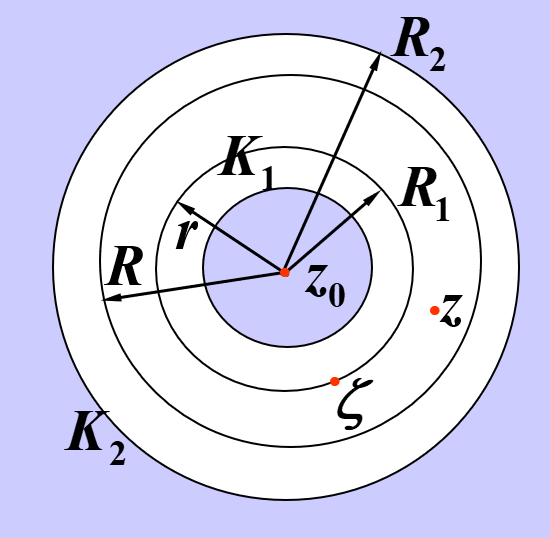
\includegraphics[width=\linewidth]{Figure_4_3_1.png}
      \end{figure}
    \end{minipage}
  \end{block}
  \begin{proofs}<2->
    For the first integral: $\frac{1}{2\pi i}\oint_{K_2}\frac{f(\zeta)}{\zeta-z}\dif\zeta$.\\
    $\begin{aligned}
        \frac{1}{\zeta-z} & =\frac{1}{(\zeta-z_0)-(z-z_0)}=\frac{-1}{z-z_0}\cdot\frac{1}{1-\frac{z-z_0}{\zeta-z_0}}\ \left(\left|\frac{z-z_0}{\zeta-z_0}\right|<1\right) \\
                          & =\frac{1}{\zeta-z_0}\sum_{n=0}^{\infty}\left(\frac{z-z_0}{\zeta-z_0}\right)^n=\sum_{n=0}^{\infty}\frac{(z-z_0)^n}{(\zeta-z_0)^{n+1}},
      \end{aligned}$
  \end{proofs}
\end{frame}

\begin{frame}
  \begin{proofs}[\proofname\ (Cont.)]
    $\begin{aligned}
        \frac{1}{2\pi i}\oint_{K_2}\frac{f(\zeta)}{\zeta-z}\dif\zeta & =\sum_{n=0}^{\infty}\left[\frac{1}{2\pi i}\oint_{K_2}\frac{f(\zeta)}{(\zeta-z_0)^{n+1}}\dif\zeta\right](z-z_0)^n \\
                                                                     & =\sum_{n=0}^{\infty}c_n(z-z_0)^n.
      \end{aligned}$\\
    For the second integral: $\frac{1}{2\pi i}\oint_{K_1}\frac{f(\zeta)}{\zeta-z}\dif\zeta$.\\
    $\begin{aligned}[t]
        \frac{1}{\zeta-z} & =\frac{1}{(\zeta-z_0)-(z-z_0)}                                                                                         \\
                          & =\frac{-1}{z-z_0}\cdot\frac{1}{1-\frac{z-z_0}{\zeta-z_0}}\ \left(\left|\frac{\zeta-z_0}{z-z_0}\right|<1\right)         \\
                          & =-\sum_{n=1}^{\infty}\frac{(\zeta-z_0)^{n-1}}{(z-z_0)^n}=-\sum_{n=1}^{\infty}\frac{1}{(\zeta-z_0)^{-n+1}}(z-z_0)^{-n},
      \end{aligned}$
  \end{proofs}
\end{frame}

\begin{frame}
  \begin{proofs}[\proofname\ (Cont.)]
    Therefore $\begin{aligned}[t]
          & -\frac{1}{2\pi i}\oint_{K_1}\frac{f(\zeta)}{\zeta-z}\dif\zeta                                                            \\
        = & \sum_{n=1}^{N-1}\left[\frac{1}{2\pi i}\oint_{K_1}\frac{f(\zeta)}{(\zeta-z_0)^{-n+1}}\dif\zeta\right](z-z_0)^{-n}+R_N(z),
      \end{aligned}$\\
    where $R_N(z)=\frac{1}{2\pi i}\oint_{K_1}\left[\sum_{n=N}^{\infty}\frac{(\zeta-z_0)^{n-1}f(\zeta)}{(z-z_0)^n}\right]\dif\zeta$.
  \end{proofs}
\end{frame}

\begin{frame}
  \begin{proofs}[\proofname\ (Cont.)]
    Let's prove that $\lim_{N\to\infty}R_N(z)=0$ holds outside $K_1$.\\
    Let $q=\left|\frac{\zeta-z_0}{z-z_0}\right|=\frac{r}{|z-z_0|}$ be independent of the integral variable $\zeta$ and $0<q<1$.\\
    Because $|f(\zeta)|\leq M$ (continuity of $f(z)$),\\
    $\begin{aligned}
        |R_N(z)| & \leq\frac{1}{2\pi}\oint_{K_1}\left[\sum_{n=N}^{\infty}\frac{|f(\zeta)|}{|\zeta-z_0|}\left|\frac{\zeta-z_0}{z-z_0}\right|^n\right]\dif s \\
                 & \leq\frac{1}{2\pi}\cdot\sum_{n=N}^{\infty}\frac{M}{r}q^n\cdot 2\pi r=\frac{Mq^N}{1-q}.
      \end{aligned}$\\
    $\lim_{N\to\infty}R_N(z)=0$ holds.
  \end{proofs}
\end{frame}

\begin{frame}
  \begin{proofs}[\proofname\ (Cont.)]
    $\begin{aligned}
        -\frac{1}{2\pi i}\oint_{K_1}\frac{f(\zeta)}{\zeta-z}\dif\zeta & =\sum_{n=1}^{\infty}\left[\frac{1}{2\pi i}\oint_{K_1}\frac{f(\zeta)}{(\zeta-z_0)^{-n+1}}\dif\zeta\right](z-z_0)^{-n} \\
                                                                      & =\sum_{n=1}^{\infty}c_{-n}(z-z_0)^{-n},
      \end{aligned}$\\
    $\begin{aligned}
        f(z) & =\frac{1}{2\pi i}\oint_{K_2}\frac{f(\zeta)}{\zeta-z}\dif\zeta-\frac{1}{2\pi i}\oint_{K_1}\frac{f(\zeta)}{\zeta-z}\dif\zeta \\
             & =\sum_{n=0}^{\infty}c_n(z-z_0)^n+\sum_{n=1}^{\infty}c_{-n}(z-z_0)^{-n}                                                     \\
             & =\sum_{n=-\infty}^{\infty}c_n(z-z_0)^n.
      \end{aligned}$
  \end{proofs}
\end{frame}

\begin{frame}
  \begin{proof}[\proofname\ (Cont.)]
    If $C$ is any positive simple closed curve around $z_0$ in the annulus. Then $c_n$ and $c_{-n}$ can be expressed as
    \[c_n=\frac{1}{2\pi i}\oint_C \frac{f(\zeta)}{(\zeta-z_0)^{n+1}}\dif\zeta,\ (n=0,\pm 1,\pm 2,\cdots).\]
  \end{proof}
\end{frame}

\begin{frame}
  \begin{block}{Note}
    \begin{enumerate}
      \item Laurent series: $f(z)=\sum_{n=-\infty}^{\infty}c_n(z-z_0)^n$
      \item The power series with positive and negative powers of the analytic function in the annulus is unique, which is the Laurent series of $f(z)$.
    \end{enumerate}
    Laurent's theorem gives a general method to expand the analytic functions in the annulus domain into Laurent series.
  \end{block}
\end{frame}

\begin{frame}
  \begin{enumerate}
    \setcounter{enumi}{2}
    \item \textbf{Laurent Expansion of Functions}
          \begin{enumerate}[1)]
            \item Direct Method\\
                  Using Laurent's theorem, the coefficients can be calculated directly:
                  \[c_n=\frac{1}{2\pi i}\oint_C \frac{f(\zeta)}{(\zeta-z_0)^{n+1}}\dif\zeta,\ (n=0,\pm 1,\pm 2,\cdots)\]
                  and $f(z)=\sum_{n=-\infty}^{\infty}c_n(z-z_0)^n$.\\
                  Disadvantages: The calculation is complicated.
          \end{enumerate}
  \end{enumerate}
\end{frame}

\begin{frame}
  \begin{enumerate}
    \item []
          \begin{enumerate}[1)]
            \setcounter{enumii}{1}
            \item Indirect Method\\
                  According to the uniqueness of the power series composed of positive and negative powers, algebraic operation, substitution, derivation and integration can be used to expand the function into Laurent series.\\
                  Advantages: It is simple and fast if it can be applied.
          \end{enumerate}
  \end{enumerate}
\end{frame}

\begin{frame}
  \begin{enumerate}
    \setcounter{enumi}{3}
    \item \textbf{Example}
  \end{enumerate}
  \begin{example}
    Expand $f(z)=\frac{e^z}{z^2}$ into a Laurent series in $0<|z|<\infty$.
  \end{example}
  \begin{solution}<2->
    According to Laurent's theorem, $f(z)=\sum_{n=-\infty}^{\infty}c_nz^n$,\\
    where $c_n=\frac{1}{2\pi i}\oint_C\frac{f(\zeta)}{(\zeta-z_0)^{n+1}}\dif\zeta=\frac{1}{2\pi i}\oint_C\frac{e^\zeta}{\zeta^{n+3}}\dif\zeta$ and $C:|z|=\rho\ (0<\rho<\infty),\ (n=0,\pm 1,\pm 2,\cdots)$.
  \end{solution}
\end{frame}

\begin{frame}
  \begin{solution}[Solution\ (Cont.)]
    When $n\leq 3$, according to Cauchy's theorem, $c_n=0$.\\
    When $n>-3$, according to Cauchy's integral formula for derivatives,\\
    $c_n=\frac{1}{2\pi i}\oint_C\frac{e^\zeta}{\zeta^{n+3}}\dif\zeta=\frac{1}{(n+2)!}\cdot\left[\frac{\dif^{n+2}}{\dif z^{n+2}}\left(e^z\right)\right]_{z=0}=\frac{1}{(n+2)!}$.\\
    So $f(z)=\sum_{n=-2}^{\infty}\frac{z^n}{(n+2)!}=\frac{1}{z^2}+\frac{1}{z}+\frac{1}{2!}+\frac{z}{3!}+\frac{z^2}{4!}+\cdots\ (0<|z|<\infty)$.
  \end{solution}
\end{frame}

\begin{frame}
  \begin{solution}[Solution\ (Cont.)]
    Another solution:\\
    $\begin{aligned}
        \frac{e^z}{z^2} & =\frac{1}{z^2}\left(1+z+\frac{z^2}{2!}+\frac{z^3}{3!}+\frac{z^4}{4!}+\cdots\right) \\
                        & =\frac{1}{z^2}+\frac{1}{z}+\frac{1}{2!}+\frac{z}{3!}+\frac{z^2}{4!}+\cdots
      \end{aligned}$\\
    \ \\
    In this example, the center $z=0$ of the annulus is not only the singularity of each negative power term, but also the singularity of $\frac{e^z}{z^2}$.
  \end{solution}
\end{frame}

\begin{frame}
  \begin{example}
    Expand $f(z)=\frac{1}{(z-1)(z-2)}$ into Laurent series in the given domains.
    \begin{minipage}{0.33\linewidth} 
      \begin{enumerate}
        \item $0<|z|<1$;
      \end{enumerate}
    \end{minipage}\begin{minipage}{0.33\linewidth}
      \begin{enumerate}
        \setcounter{enumi}{1}
        \item $1<|z|<2$;
      \end{enumerate}
    \end{minipage}\begin{minipage}{0.33\linewidth}
      \begin{enumerate}
        \setcounter{enumi}{2}
        \item $2<|z|<+\infty$.
      \end{enumerate}
    \end{minipage}
  \end{example}
  \begin{solution}<2->
    $f(z)=\frac{1}{1-z}-\frac{1}{2-z}$
  \end{solution}
\end{frame}

\begin{frame}
  \begin{solution}[Solution\ (Cont.)]
    \begin{enumerate}
      \item \begin{minipage}[t]{0.7\linewidth}\vspace{0pt}%
              $0<|z|<1$.\\
              $|z|<1\Longrightarrow\left|\frac{z}{2}\right|<1$\\
              $\frac{1}{1-z}=1+z+z^2+\cdots+z^n+\cdots$
            \end{minipage}\begin{minipage}[t]{0.3\linewidth}\vspace{0pt}%
              \begin{tikzpicture}[scale=0.7]
                \draw [gray,fill=cyan] (0,0) circle [radius=1];
                \draw [->] (-1.5,0) -- (1.5,0) node [below] {$x$};
                \draw [->] (0,-1.5) -- (0,1.5) node [below right] {$y$};
                \node [below left] at (0,0) {$O$};
                \node [below,xshift=3] at (1,0) {1};
              \end{tikzpicture}
            \end{minipage}\\
            $\frac{1}{2-z}=\frac{1}{2}\cdot\frac{1}{1-\frac{z}{2}}=\frac{1}{2}\left(1+\frac{z}{2}+\frac{z^2}{2^2}+\cdots+\frac{z^n}{2^n}+\cdots\right)$\\
            $\begin{aligned}
                f(z) & =\left(1+z+z^2+\cdots\right)+\frac{1}{2}\left(1+\frac{z}{2}+\frac{z^2}{2^2}+\cdots\right) \\
                     & =\frac{1}{2}+\frac{3}{4}z+\frac{7}{8}z^2+\cdots
              \end{aligned}$
    \end{enumerate}
  \end{solution}
\end{frame}

\begin{frame}
  \begin{solution}[Solution\ (Cont.)]
    \begin{enumerate}
      \setcounter{enumi}{1}
      \item \begin{minipage}[t]{0.7\linewidth}\vspace{0pt}%
              $1<|z|<2$.\\
              $|z|>1\Longrightarrow\left|\frac{1}{z}\right|<1$\\
              $|z|<2\Longrightarrow\left|\frac{z}{2}\right|<1$
            \end{minipage}\begin{minipage}[t]{0.3\linewidth}\vspace{0pt}%
              \begin{tikzpicture}[scale=0.7]
                \draw [gray,fill=cyan] (0,0) circle [radius=1];
                \draw [gray,fill=white] (0,0) circle [radius=0.5];
                \draw [->] (-1.5,0) -- (1.5,0) node [below] {$x$};
                \draw [->] (0,-1.5) -- (0,1.5) node [below right] {$y$};
                \node [below left] at (0,0) {$O$};
                \node [below,xshift=3] at (0.5,0) {1};
                \node [below,xshift=3] at (1,0) {2};
              \end{tikzpicture}
            \end{minipage}\\
            $\frac{1}{1-z}=-\frac{1}{z}\cdot\frac{1}{1-\frac{1}{z}}=-\frac{1}{z}\left(1+\frac{1}{z}+\frac{1}{z^2}+\cdots+\frac{1}{z^n}+\cdots\right)$\\
            $\frac{1}{2-z}=\frac{1}{2}\cdot\frac{1}{1-\frac{z}{2}}=\frac{1}{2}\left(1+\frac{z}{2}+\frac{z^2}{2^2}+\cdots+\frac{z^n}{2^n}+\cdots\right)$\\
            $\begin{aligned}
                f(z) & =-\frac{1}{z}\left(1+\frac{1}{z}+\frac{1}{z^2}+\cdots\right)-\frac{1}{2}\left(1+\frac{z}{2}+\frac{z^2}{2^2}+\cdots\right) \\
                     & =\cdots-\frac{1}{z^n}-\frac{1}{z^{n-1}}-\cdots-\frac{1}{z}-\frac{1}{2}-\frac{z}{4}-\frac{z^2}{8}-\cdots
              \end{aligned}$
    \end{enumerate}
  \end{solution}
\end{frame}

\begin{frame}
  \begin{solution}[Solution\ (Cont.)]
    \begin{enumerate}
      \setcounter{enumi}{2}
      \item \begin{minipage}[t]{0.7\linewidth}\vspace{0pt}%
              $2<|z|<\infty$.\\
              $|z|>2\Longrightarrow\left|\frac{1}{z}\right|<\left|\frac{2}{z}\right|<1$
            \end{minipage}\begin{minipage}[t]{0.3\linewidth}\vspace{0pt}%
              \begin{tikzpicture}[scale=0.7]
                \fill [cyan] (-1.2,-1.2) rectangle (1.2,1.2);
                \draw [gray,fill=white] (0,0) circle [radius=1];
                \draw [->] (-1.5,0) -- (1.5,0) node [below] {$x$};
                \draw [->] (0,-1.5) -- (0,1.5) node [below right] {$y$};
                \node [below left] at (0,0) {$O$};
                \node [below,xshift=3] at (0.5,0) {1};
                \node [below,xshift=3] at (1,0) {2};
              \end{tikzpicture}
            \end{minipage}\\
            $\frac{1}{1-z}=-\frac{1}{z}\cdot\frac{1}{1-\frac{1}{z}}=-\frac{1}{z}\left(1+\frac{1}{z}+\frac{1}{z^2}+\cdots+\frac{1}{z^n}+\cdots\right)$\\
            $\frac{1}{2-z}=-\frac{1}{z}\cdot\frac{1}{1-\frac{2}{z}}=-\frac{1}{z}\left(1+\frac{2}{z}+\frac{2^2}{z^2}+\cdots+\frac{2^n}{z^n}+\cdots\right)$\\
            $\begin{aligned}
                f(z) & =-\frac{1}{z}\left(1+\frac{1}{z}+\frac{1}{z^2}+\cdots\right)+\frac{1}{z}\left(1+\frac{2}{z}+\frac{2^2}{z^2}+\cdots\right) \\
                     & =\frac{1}{z^2}+\frac{3}{z^3}+\frac{7}{z^4}+\cdots
              \end{aligned}$
    \end{enumerate}
  \end{solution}
\end{frame}

\begin{frame}
  \begin{solution}[Solution\ (Cont.)]
    In this example, the center $z=0$ of the annulus domain is the singularity of each negative power term, but not the singularity of $f(z)=\frac{1}{(z-1)(z-2)}$.
  \end{solution}
  \begin{block}{Note}
    \begin{enumerate}
      \item Although the $f(z)$ contains the negative power term of $z-z_0$ in the Laurent series in the annulus domain centered on $z_0$, and $z_0$ is the singularity of these terms, $z_0$ may or may not be the singularity of function $f(z)$.
    \end{enumerate}
  \end{block}
\end{frame}

\begin{frame}
  \begin{block}{Note}
    \begin{enumerate}
      \setcounter{enumi}{1}
      \item Given the function $f(z)$ and a point in the complex plane, the function has different Laurent expansions in different annulus domains (including Taylor expansion as its special case).
    \end{enumerate}
  \end{block}
  \begin{block}{Question}
    Does this contradict the uniqueness of Laurent's expansion?
  \end{block}
  \begin{block}{Answer}<2->
    No contradiction. (Uniqueness: it means that the Laurent expansion of a function in a given annulus domain is unique)
  \end{block}
\end{frame}

\begin{frame}
  \begin{example}
    Expand $f(z)=\frac{\sin z}{z}$ in a Laurent series about $z_0=0$.
  \end{example}
  \begin{solution}<2->
    $\begin{aligned}
        f(z) & =\frac{\sin z}{z}                                                                                       \\
             & =\frac{1}{z}\left[z-\frac{1}{3!}z^3+\frac{1}{5!}z^5-\cdots+(-1)^n\frac{z^{2n+1}}{(2n+1)!}+\cdots\right] \\
             & =\sum_{n=0}^{\infty}\frac{(-1)^nz^{2n}}{(2n+1)!}\ (0<|z|<\infty)
      \end{aligned}$
  \end{solution}
\end{frame}

\begin{frame}
  \begin{example}
    Compute the integral $\oint_Cf(z)\dif z$, where $C$ is the circle $|z|=3$ taken counterclockwise and $f(z)=\frac{1}{z(z+1)^2}$.
  \end{example}
  \begin{solution}<2->
    $\begin{aligned}
        f(z) & =\frac{1}{z(z+1)^2}=\frac{1}{z}\cdot\left(\frac{-1}{1+z}\right)'=-\frac{1}{z}\left(\frac{1}{z}\cdot\frac{1}{1+\frac{1}{z}}\right)' \\
             & =-\frac{1}{z}\left[\frac{1}{z}\cdot\left(1-\frac{1}{z}+\frac{1}{z^2}-\cdots\right)\right]'                                         \\
             & =-\frac{1}{z}\left(-\frac{1}{z^2}+\frac{2}{z^3}-\frac{3}{z^4}-\cdots\right)=\frac{1}{z^3}-\frac{2}{z^4}+\cdots
      \end{aligned}$
  \end{solution}
\end{frame}

\begin{frame}
  \begin{solution}[Solution\ (Cont.)]
    Because $c_n=\frac{1}{2\pi i}\oint_C\frac{f(\zeta)}{(\zeta-z_0)^{n+1}}\dif\zeta$,\\
    $c_{-1}=\frac{1}{2\pi i}\oint_Cf(\zeta)\dif\zeta\Longrightarrow\oint_Cf(\zeta)\dif\zeta=2\pi ic_{-1}$,\\
    $\oint_C\frac{1}{z(z+1)^2}\dif z=0$.
  \end{solution}
\end{frame}

\begin{frame}
  \begin{example}
    Compute the integral $\oint_{|z|=\frac{1}{2}}\frac{e^\frac{1}{z}}{1-z}\dif z$.
  \end{example}
  \begin{solution}<2->
    \resizebox*{\linewidth}{!}{$\frac{e^\frac{1}{z}}{1-z}=\left(1+z+z^2+\cdots+z^n+\cdots\right)\left(1+\frac{1}{z}+\frac{1}{2!z^2}+\cdots+\frac{1}{n!z^n}+\cdots\right)$}\\
    $c_{-1}=1+\frac{1}{2!}+\frac{1}{3!}+\cdots+\frac{1}{n!}+\cdots=e-1$\\
    $\oint_{|z|=\frac{1}{2}}\frac{e^\frac{1}{z}}{1-z}\dif z=2\pi i(e-1)$
  \end{solution}
\end{frame}

\begin{frame}
  \begin{enumerate}
    \setcounter{enumi}{4}
    \item \textbf{Summary and Thinking}\\
          In this part, we learned about the Laurent expansion theorem and the method of expanding functions into Laurent series. The expansion of functions into Laurent series is the key and difficult point of this part.
  \end{enumerate}
\end{frame}

\begin{frame}
  \begin{block}{Question}
    What is the relationship between Laurent series and Taylor series?
  \end{block}
  \begin{block}{Answer}<2->
    It is the relationship between the general and the special.\\
    Laurent series is a two-side power series, and its analytic part is a common power series. The region of convergence of Laurent series is annulus $r<|z-z_0|<R$.\\
    When $r=0,c_{-n}=0$, the Laurent series degenerates into the Taylor series.
  \end{block}
\end{frame}

\end{document}
